\section{介绍}

在Python的\href{https://wiki.python.org/moin/ParallelProcessing}{wiki列表}中,存在许多与Python相关的库,可用于在对称多处理(SMP)或共享内存环境中使用多个CPU或多核CPU以及在群集或网格环境中使用大量计算机。

与SMP体系结构不同,尤其是与基于线程的并发相反,群集(和网格)体系结构由于相对缺乏共享资源而提供了高可伸缩性,尽管这会使编程范式对于未开始的开发人员而言似乎有些陌生。在此域中,可能会发现与其他分布式计算技术有一些重叠。

\subsection{分布式集群框架}
下面介绍几个常用的分布式集群框架。

\subsubsection{ParallelPython}
\href{https://www.parallelpython.com/}{ParallelPython}是一个是用纯Python编写的开源和跨平台模块,提供了在SMP(具有多个处理器或核心的系统)和群集(通过网络连接的计算机)上并行执行python代码的机制。它比较轻巧,易于安装并与其他python软件集成。具有以下一些特征:
\begin{itemize}
    \item 可在SMP和集群上并行执行python代码
    \item 易于理解和实现基于作业的并行化技术(易于并行转换串行应用程序)
    \item 可自动检测最佳配置(默认情况下,工作进程数设置为有效处理器数)
    \item 可动态处理器分配(工作进程数可以在运行时更改)
    \item 具有相同功能的后续作业的开销很低(实现透明缓存以减少开销)
    \item 可动态负载平衡(作业在运行时在处理器之间分配)
    \item 容错(如果其中一个节点失败,则将任务重新安排到其他节点上)
    \item 可自动发现计算资源
    \item 可动态分配计算资源(自动发现和容错的后果)
    \item 基于SHA的网络连接身份验证
    \item 跨平台的可移植性和互操作性(Windows,Linux,Unix,Mac OS X)
    \item 跨体系结构的可移植性和互操作性(x86,x86-64等)
    \item 开源
\end{itemize}

该开源框架存在的不足之处在于开发版本较少,且大部分版本基于python2.开发,而DETRIA程序的代码是为python3.。因此,在调用该模块需更改大量代码并且可能遇到因python3.不向下兼容而导致无法调用的情况。图\ref{ParallelPython分布式计算}为ParallelPython实现简单分布式程序的结果。

\begin{figure}[h]
    \centering
    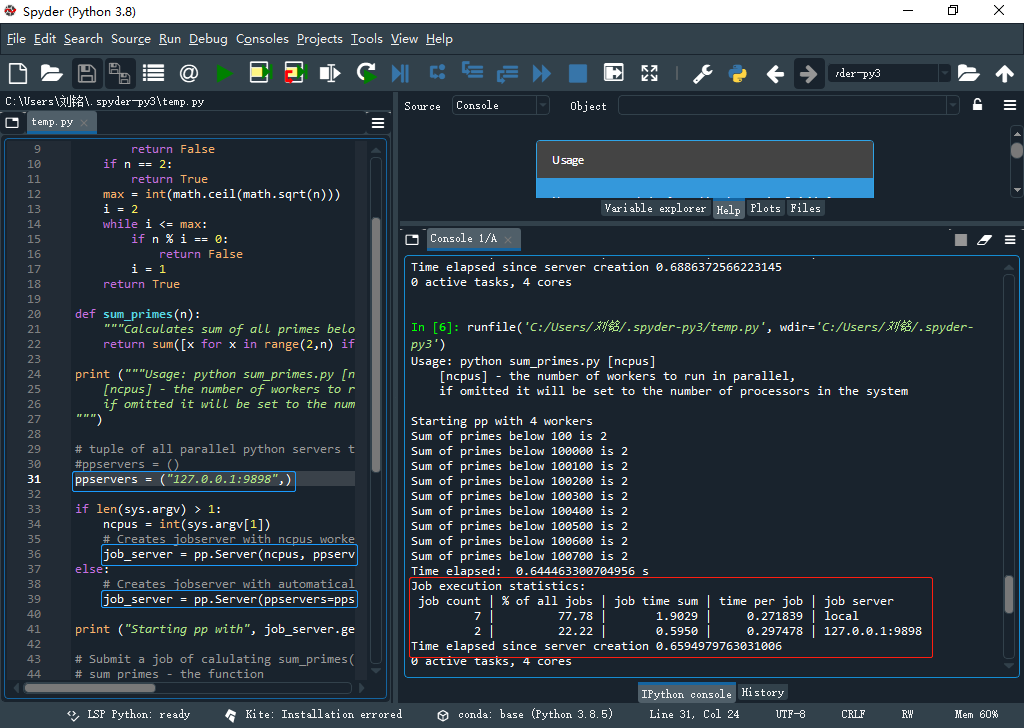
\includegraphics[width=1.0\textwidth]{ParallelPython.png}
    \caption{ParallelPython分布式计算}
    \label{ParallelPython分布式计算}
\end{figure}

\subsubsection{Dask}
\href{https://dask.org/}{Dask}是用于Python中并行计算的灵活库,该库由两部分组成:
\begin{enumerate}
    \item 动态任务调度针对计算进行了优化。这类似于 Airflow,Luigi,Celery或Make,但针对交互式计算工作负载进行了优化。
    \item “大数据”集合(例如并行数组,数据框和列表)将诸如NumPy,Pandas或Python迭代器之类的通用接口扩展到了大于内存或分布式的环境。这些并行集合在动态任务计划程序之上运行。
\end{enumerate}
Dask有以下特点:
\begin{itemize}
    \item Familiar:提供并行的NumPy数组和Pandas DataFrame对象
    \item Flexible:提供任务计划界面,用于更多自定义工作负载并与其他项目集成
    \item Native:在纯Python中启用分布式计算,并可以访问PyData堆栈
    \item Fast:以低开销,低延迟和快速数值算法所需的最少序列化操作
    \item Scales up:在具有1000个核心的集群上弹性运行
    \item Scales down:在单个过程中轻松设置并在笔记本电脑上运行
    \item Responsive:设计时考虑了交互式计算,它提供了快速的反馈和诊断功能,以帮助用户
\end{itemize}

Dask分布式框架提供了丰富的集群配置方法:1)\href{https://docs.dask.org/en/latest/setup/cli.html}{命令行设置};2)\href{https://docs.dask.org/en/latest/setup/ssh.html}{SSH配置};3)\href{https://docs.dask.org/en/latest/setup/hpc.html}{使用MPI等工具在传统HPC环境中配置};4)\href{https://docs.dask.org/en/latest/setup/kubernetes.html}{通过流行的Kubernetes资源管理器部署};5)\href{https://yarn.dask.org/en/latest/}{在YARN群集上部署};6)\href{https://docs.dask.org/en/latest/setup/python-advanced.html}{自定义Python的API};7)\href{https://docs.dask.org/en/latest/setup/docker.html}{Docker容器};8)\href{https://docs.dask.org/en/latest/setup/cloud.html}{在常见云服务器上部署}。图\ref{Dask集群Dashboard}是通过命令行方式配置的Dask集群。
\begin{figure}[h]
    \centering
    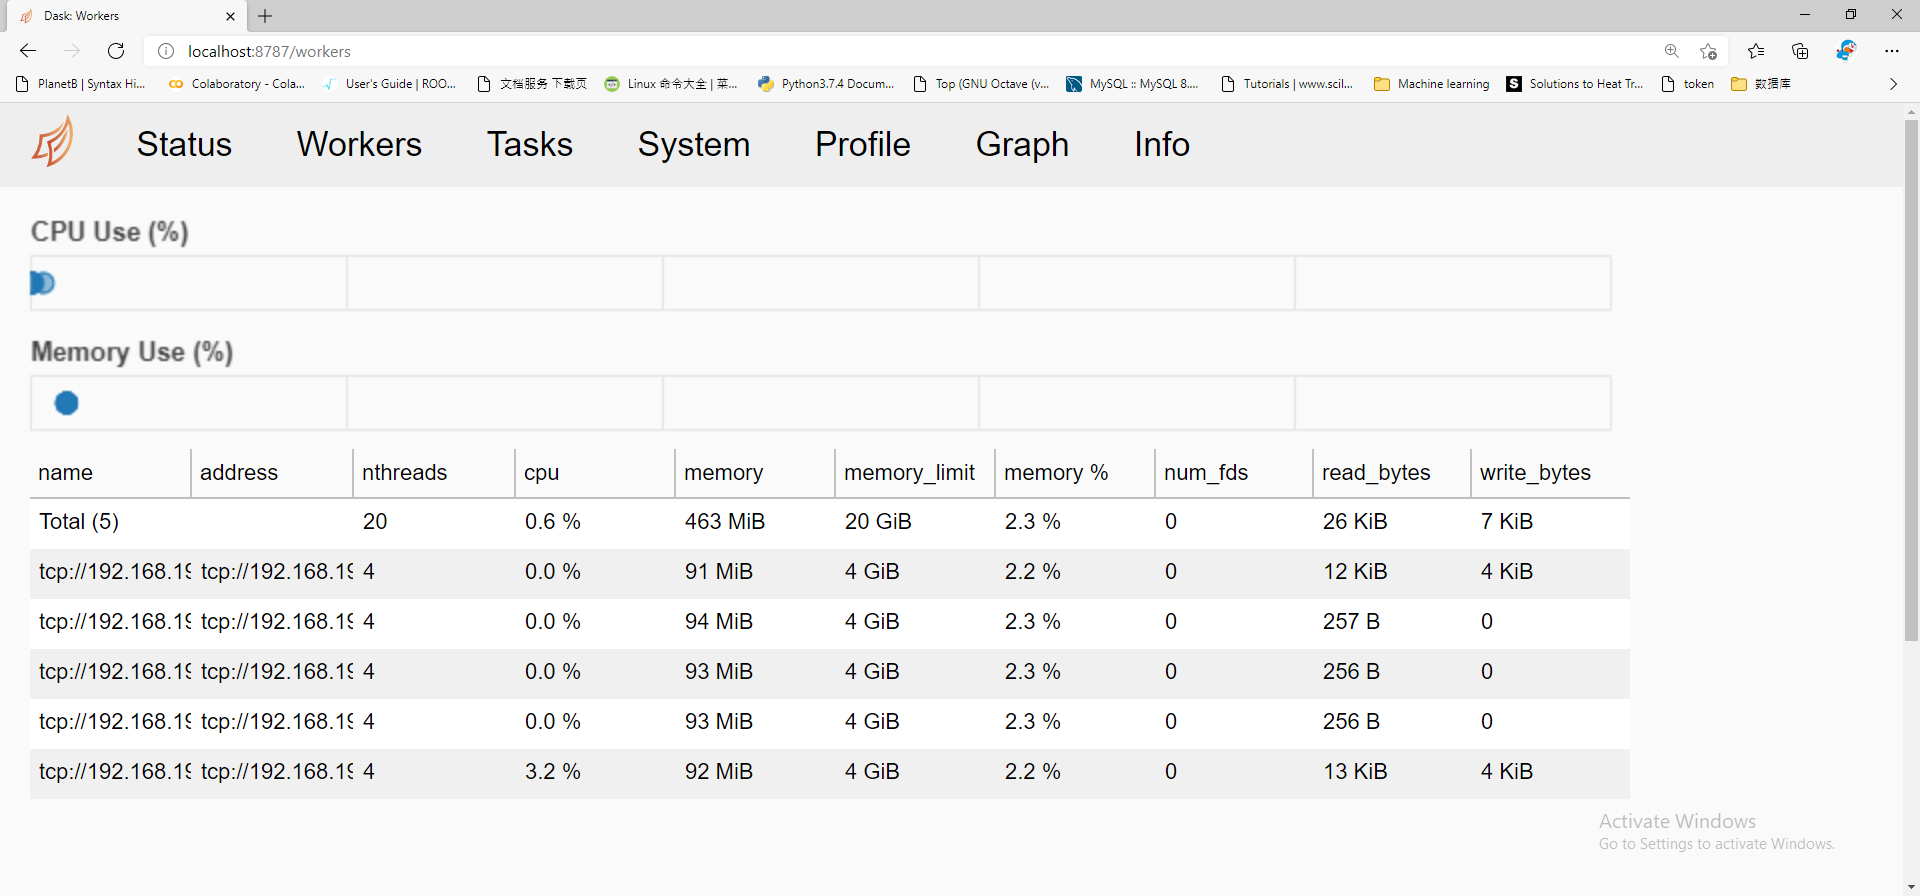
\includegraphics[width=1.0\textwidth]{Dask.png}
    \caption{Dask集群Dashboard}
    \label{Dask集群Dashboard}
\end{figure}

\subsubsection{mpi4py}
\href{https://pypi.org/project/mpi4py/}{mpi4py}(MPI for python)是一个构建在MPI之上的Python库,它使得Python的数据结构可以方便的在多进程中传递。它实现了很多MPI标准中的接口,包括点对点通信、集合通信、阻塞/非阻塞通信、组间通信等,基本上能用到的MPI接口都有相应的实现。而\href{https://www.open-mpi.org/}{MPI}是一种标准化的和便携式的消息传递系统,其设计功能上各种各样的并行计算机。虽然mpi4py是一个框架库,但是其本质仅仅是为了用户在编写python程序时更加方便的调用MPI接口而包装的一个框架。因此,在使用mpi4py时,需要用户在计算机中安装MPICH或Open MPI。

所以,尽管mpi4py在理论上可以实现分布式集群环境的搭建,但是相比于现有其他强大的python库,mpi4py需要用户自己编写更加底层的代码,再者DETRIA程序的整体已经编写完成,若要使用mpi4py搭建分布式集群计算,需要从程序开发框架上重新编写,工作量较大。综上,mpi4py不考虑作为DETRIA的集群计算环境搭建框架。

\subsubsection{Ray}
\href{https://ray.io/}{Ray}提供了用于构建分布式应用程序的简单通用API。Ray的工作是确保应用程序能够以分布式方式运行,并具有分布式计算所需的所有节点内通信、数据传输和抗故障能力。Ray具有以下特征:
\begin{enumerate}
    \item 提供用于构建和运行分布式应用程序的简单API
    \item 使用户能够并行化仅在单台机器编写代码,几乎不用更改代码
    \item 在核心Ray之上包括一个大型的应用程序、库和工具生态系统,以支持复杂的应用程序
\end{enumerate}

但是,Ray当前支持MacOS和Linux。现在Windows稳定版暂时未推出,但是有Windows试验版并且正在开发中。图\ref{Ray在Ubuntu系统上搭建集群环境}为Ray在Linux系统上搭建的集群环境。
\begin{figure}[h]
    \centering
    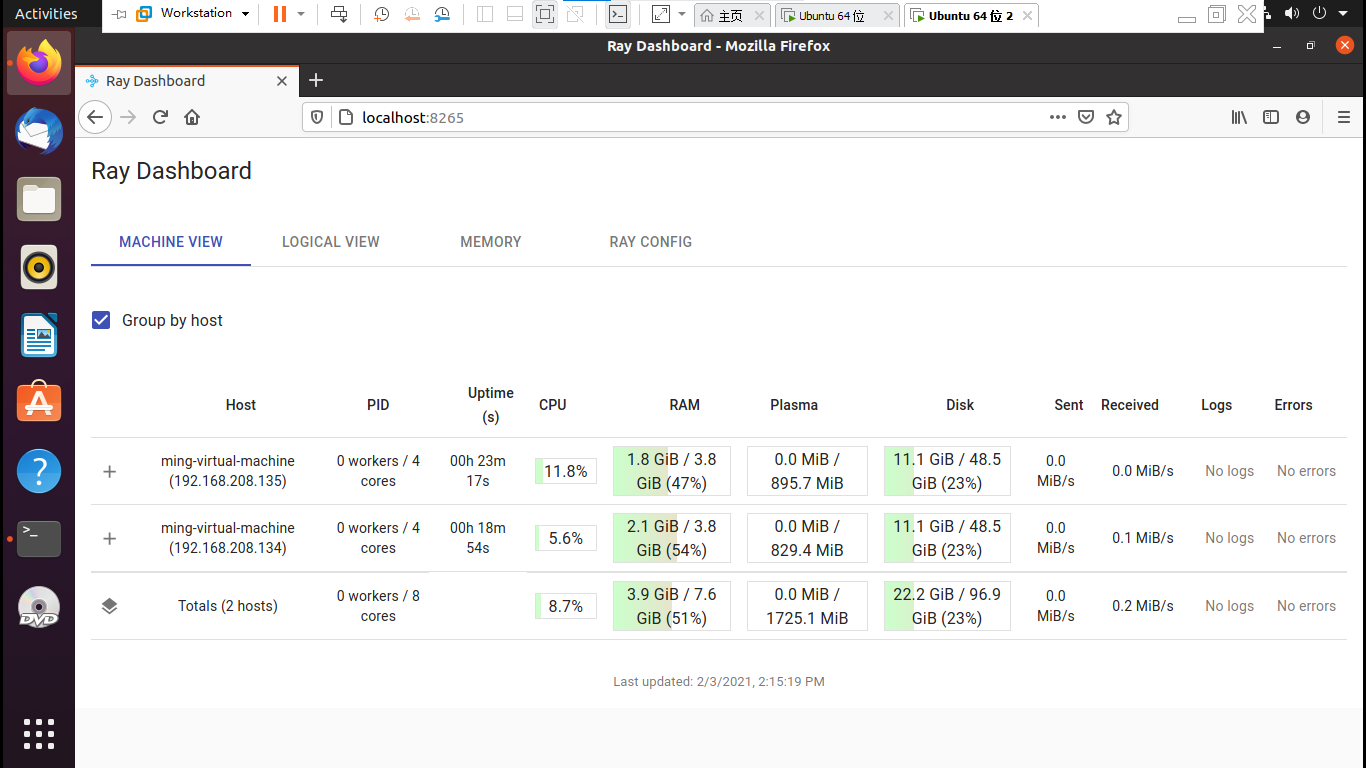
\includegraphics[width=0.9\textwidth]{RayDashboard.png}
    \caption{Ray在Ubuntu系统上搭建集群环境}
    \label{Ray在Ubuntu系统上搭建集群环境}
\end{figure}

除了上述介绍的几种分布式框架外,Python还有非常多分布式集群库,例如\href{https://pypi.org/project/pathos/}{pathos}、\href{https://pypi.org/project/celery/}{celery}、\href{http://www.inspirel.com/yami4/}{yami4}等等。